\chapter{Implementation}

\section{Complete Workflow of the System:}




\section{The Grammar of Annotation Language:}
Figure 4.1 contains in Extended Backus Naur Form (EBNF) notation the grammar of our annotation language. The following type face conventions were used: Italic font for non-terminals, bold typewriter font for literal terminals including keywords.
Our annotation language grammar has two grammar rules
\texttt{S\_L\_Anno} and \texttt{M\_L\_Anno} used for defining security annotations. The \texttt{Func\_Decl} and \texttt{Attr\_Definition} rules are
used to recognize C or C++ function declarations and variable
declarations.

\begin{figure}[ht!]
	\begin{tabular}{lll}
		\footnotesize                       
		\textit{Ann\_Lang}           &\footnotesize $::=$         &\footnotesize HeaderModel*;       \\ \\
		
		\footnotesize
		\textit{H\_Model}            &\footnotesize $::=$         &\footnotesize \textit{S\_L\_Anno};       \hfill ;single line comment rule   \\     
		&\footnotesize $\ \vert $    &\footnotesize \textit{M\_L\_Anno};       \hfill ;multi line comment rule    \\ 
		&\footnotesize $\ \vert $    &\footnotesize \textit{Func\_Decl};       \hfill ;function declaration rule  \\ 
		&\footnotesize $\ \vert $    &\footnotesize \textit{Attr\_Def};        \hfill ;variable declaration rule  \\ \\
		\footnotesize  	
		\textit{S\_L\_Anno}          &\footnotesize $::=$         &\footnotesize \textbf{"//@ @function "},    Func\_Type,              [\textbf{H} $\ \vert $  \textbf{L}];     \\
		&\footnotesize $\ \vert $    &\footnotesize \textbf{"//@ @parameter "},   p\_Name,  Sec\_Type, Var\_Type,    [\textbf{H} $\ \vert $  \textbf{L}];    \\
		&\footnotesize $\ \vert $    &\footnotesize \textbf{"//@ @variable "},    v\_Name,  Sec\_Type,     [\textbf{H} $\ \vert $  \textbf{L}];    \\
		&\footnotesize $\ \vert $    &\footnotesize \textbf{"//@ @preStep "},     pr\_s\_Name,             [\textbf{H} $\ \vert $  \textbf{L}];    \\
		&\footnotesize $\ \vert $    &\footnotesize \textbf{"//@ @postStep "},    po\_s\_Name,             [\textbf{H} $\ \vert $  \textbf{L}];    \\ \\   
		\footnotesize            
		\textit{M\_L\_Anno}          &\footnotesize $::=$         &\footnotesize [\textbf{"/*@ "}],  ["* "],  Func\_Ann,  (\textbf{" @*/"}) \\
		&\footnotesize $\ \vert $    &\footnotesize ("*"), [" "]*, (\textbf{"@*/"});                  \\ \\
		\footnotesize        
		\textit{Func\_Ann}           &\footnotesize $::=$         &\footnotesize \textbf{"@function "},    Func\_Type,              [\textbf{H} $\ \vert $  \textbf{L}];     \\
		&\footnotesize $\ \vert $    &\footnotesize \textbf{"@parameter "},   p\_Name,  Sec\_Type, Var\_Type,    [\textbf{H} $\ \vert $  \textbf{L}];    \\
		&\footnotesize $\ \vert $    &\footnotesize \textbf{"@preStep "},     pr\_s\_Name,             [\textbf{H} $\ \vert $  \textbf{L}];    \\
		&\footnotesize $\ \vert $    &\footnotesize \textbf{"@postStep "},    po\_s\_Name,             [\textbf{H} $\ \vert $  \textbf{L}];    \\ \\                                        
		\footnotesize                       
		\textit{Func\_Type}          &\footnotesize $::=$        &\footnotesize \textbf{authentication};\\
		 &\footnotesize $\ \vert $ &\footnotesize \textbf{declassification}; \\
		&\footnotesize $\ \vert $    &\footnotesize \textbf{sanitization};     \\
		&\footnotesize $\ \vert $    &\footnotesize \textbf{sink};             \\
		&\footnotesize $\ \vert $    &\footnotesize \textbf{source};           \\
		&\footnotesize $\ \vert $    &\footnotesize \textbf{trust\_boundary};  \\ \\
		\footnotesize                       
		\textit{Sec\_Type}           &\footnotesize $::=$         &\footnotesize \textbf{confidential}; \\
		&\footnotesize $\ \vert $    &\footnotesize \textbf{source};    \\ \\
		\footnotesize                       
		\textit{Var\_Type}           &\footnotesize $::=$         &\footnotesize \textbf{authenticated}; \\
		&\footnotesize $\ \vert $    &\footnotesize \textbf{declassified}
		\\
		&\footnotesize $\ \vert $    &\footnotesize \textbf{sanitized};    \\ \\	
		                       
	\end{tabular}
	\caption{Light-weight annotation language grammar excerpt}
	\label{language grammar}
\end{figure}

As per requirements previous annotation language grammar which is written in xtext language has been extended. Extra annotation have included like \enquote{authenticated}, \enquote{declassified}, \enquote{sanitized}, \enquote{sanitization}, \enquote{declassification}, \enquote{authentication}. Some part of the code snippet of extended xtext grammar is given below.
\begin{lstlisting}
	/**
	* @FunctionAnnotation :used for function annotations
	*/ 
	FunctionAnnotation returns FunctionAnnotation:
	{FunctionAnnotation}( 
	result +=  '@function '   functionType=FunctionType      (' ')?                              (level =('H'|'L'))?     ((name0=ID))? ((nameComment=ID))? ('\n' | '\r')?
	// supported without space before confidential and sensitive
	| '@parameter '   parameter=ID (name0=ID)? (securityType=SecurityType)?(' ')?  (level =('H'|'L'))? ('True'|'False')? (variableTyp=VariableType)?  ((name1=ID))? ((nameComment=ID))? ('\n' | '\r')?	
	;
	
	/**
	* @SingleLineAnnotation :used for adding single line annotations
	*/ 
	SingleLineAnnotation returns SingleLineAnnotation:
	{SingleLineAnnotation}(
	result+=  '//@ @function '    functionType=FunctionType (' ')?                  (level =('H'|'L'))?  ((name0=ID))? ((nameComment=ID))?  ('\n' | '\r')*
	// supported without space before confidential and sensitive
	| '//@ @parameter '   parameter=ID (securityType=SecurityType)? (' ')?  (level =('H'|'L'))? ('True'|'False')? (variableTyp=VariableType)?  ((nameComment=ID))?  ('\n' | '\r')?
	| '//@ @variable '    variable=ID  (securityType=SecurityType)? (' ')?  (level =('H'|'L'))? ('True'|'False')? ((nameComment=ID))?  ('\n' | '\r')?
	
	;
	
	/**
	* @FunctionType :annotaions types for functions
	*/ 
	enum FunctionType: declassification 
	| sanitization
	| authentication
	| sink
	| source
	| trust_boundary
	;
	
	
	/**
	* @VariableSituation :annotaions types for function parameters
	*/ 
	enum VariableType: declassified 
	| sanitized
	| authenticated
	;
	
	
\end{lstlisting}

\section{UML State Chart Editor:}
UML state chart editor has been extended based on the open source Yakindu SCT \cite{ref_15_yakindu:sct}framework. The existing language grammar with
annotation language grammar has extended in order to support new set
of tags. Furthermore, an annotation proposal filter implemented which was used to filter out the annotation language tags of the Yakindu SCT language grammar.

\section{Source Code Editor:}
The source code editor has extended which offers annotation language proposals which are context sensitive with respect to the position of the currently edited syntax line.Editor suggestions work only if the whole file is parsed without errors.

\section{C Code Generator:}
C code generator has extended based on Eclipse EMF and xTend which is used to generate the state chart execution code containing the previously added security annotations from UML state charts. The code generator outputs two files per UML state chart (one .c and one
.h file). Generated annotations can reside in both header file
and source code file. Previously annotated UML state chart
states are converted to either C function calls or C variables
declarations, both have been previously annotated. We use
the available state chart execution flow functionality which is
responsible for traversing the UML state chart during state
chart simulation. The UML state chart will be traversed by the code generation algorithm and code is generated based on
the mentioned state chart execution flow. The generated code
will contain at least one bad path (contains a true positive) and
a good path (contains no bug) per UML state chart if those
paths were previously modeled inside the UML state chart.

\section{View Buggy Path in Sequence Diagram}
Through the static analysis engine buggy path can be found as a list of string. Inside the list there are function calls, separate statements like if statements, switch-case statements, variable declaration, assignment of variables etc. of programming language (like C,C++). Then to view the path using java a sequence diagram is generated.
now it easier to trace the buggy path by viewing generated sequence diagram. One sample example of the buggy path is given in figure 4.1.
\begin{figure}[htbp]
	\centering
	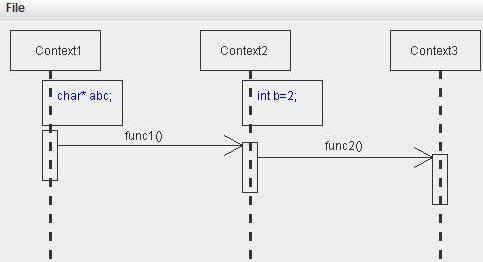
\includegraphics{styles/Error_trace_path.jpg}
	\caption{Error trace path in sequence diagram}
\end{figure}
